\section{\ix Design Approach}
\label{sec:design}

The first two requirements in \S\ref{sec:motivation:challenges} ---
microsecond latency and high packet rates --- are not unique to
web-scale applications. These requirements have been addressed in the
design of middleboxes such as firewalls, load-balancers, and software
routers~\cite{routebricks,click} by integrating the networking stack
and the application into a single \emph{dataplane}. The two remaining
requirements --- protection and resource efficiency --- are not
addressed in middleboxes because they are single-purpose systems, not
exposed directly to users.

Dataplanes differ from traditional OS designs in two basic
ways. First, they are designed to \emph{run each packet to
  completion}. All network protocol and application processing for a
packet is done before moving on to the next packet.  In contrast, a
commodity OS decouples protocol processing from the application itself
in order to provide scheduling and flow control flexibility.  For
example, the kernel relies on device and soft interrupts to context
switch from applications to protocol processing. Similarly, the
kernel's network stack will generate TCP \texttt{ACKs} and slide its
receive window even when the application is not consuming data, up to
an extent. Second, dataplanes optimize for \emph{synchronization-free
  operation} in order to scale well on many cores. Network flows are
distributed into distinct queues via flow-consistent hashing, such as
Recieve Side Scaling (RSS)~\cite{url:rss}, and common case packet processing requires no
synchronization or coherence traffic between cores.

\ix extends the dataplane architecture to support untrusted
applications and satisfy all requirements in
\S\ref{sec:motivation:challenges}. Its design is based on the
following key principles:

% \christos{this list must be aligned with 2.2. Ie we should explain how
%   each approach helps with the requirements. This is critical}

\myparagraph{Separation and protection of control and data plane:} \ix
separates the control function of the kernel, responsible for resource
configuration, provisioning, scheduling, and monitoring, from the
dataplane, which runs the networking stack and application logic.
Like a conventional OS, the control plane multiplexes and schedules
resources among dataplanes, but in a coarse-grained manner in space
and time. Entire cores are dedicated to dataplanes, memory is
allocated at large page granularity, and NIC queues are assigned to
dataplane cores. The control plane is also responsible for elastically
adjusting the allocation of resources between dataplanes.

The separation of control and data plane allows us to consider
radically different I/O APIs and implementations in the dataplane,
while permitting other OS functionality, such as file system support,
to be passed through to the control plane for compatibility.
Similar to the Exokernel~\cite{DBLP:conf/sosp/EnglerKO95}, each
dataplane runs a single application in a single address
space. However, we use modern virtualization hardware to provide
three-way isolation between the control plane, the dataplane, and
untrusted user code~\cite{dune}. Dataplanes have capabilities similar
to guest OSes in virtualized systems. They manage their own address
translations, on top of the address space provided by the control
plane, and can protect the networking stack from untrusted application
logic through the use of privilege rings. Moreover, dataplanes are
given direct pass-through access to NIC queues through memory mapped
I/O.

% \christos{we should bring up HW virtualization here, likely as a
%   independent part of the approach or merged with the one above. It is
%   a big part of the protection story. The discussion on CP/DP
%   seperation must be linked to elasticity too}


\myparagraph{Run to completion with adaptive batching:} \ix dataplanes
runs to completion all stages needed to receive and transmit a packet,
interleaving protocol processing (kernel mode) and application logic
(user mode) at well-defined transition points. Hence, there is no need
for intermediate buffering between protocol stages or between
application logic and the networking stack.  Unlike previous work, that
applied a similar approach to eliminate receive livelocks during
congestion periods~\cite{receive-livelock}, \ix uses run to completion
during all load conditions. Thus, we are able to use polling and avoid
interrupt overhead in the common case. We still rely on interrupts as
a mechanism to regain control, for example, if a dataplane is slow to
respond.  Run to completion improves both message throughput and
latency because successive stages tend to access many of the same
data, leading to better data cache locality.

The \ix dataplane also makes extensive use of batching.  Previous
systems applied batching at the system call
boundary~\cite{DBLP:conf/osdi/HanMCR12, DBLP:conf/osdi/SoaresS10} and
at the network API and hardware queue level~\cite{jeong2014mtcp}.  We
apply batching in every stage of the network stack, including but not
limited to system calls and queues. Moreover, we use batching
\emph{adaptively} as follows: (i) we never wait to batch requests and
batching only occurs in the presence of congestion; (ii) we set an
upper bound on the number of batched packets. Using batching only on
congestion allows us to minimize the impact on latency, while bounding
the batch size prevents the live set from exceeding cache capacities
and avoids transmit queue starvation. Batching improves packet rate
because it amortizes system call transition
overheads % (although these costs are
% relatively small on modern hardware)
and improves instruction cache locality, prefetching effectiveness,
and branch prediction accuracy. When applied adaptively, batching also
decreases latency because these same efficiencies reduce head-of-line
blocking.

The combination of bounded, adaptive batching and run to completion
means that queues for incoming packets can build up only at the NIC
edge, before packet processing starts in the dataplane.
% before packets are processed by the dataplane. \ana{Emphasize that
% we are not wasting resources on packets that might have to be
% dropped; drop early at the NIC if can't handle.  Citation for Mogul
% and Ramakrishnan could go here.}
The networking stack sends acknowledgments to peers only as fast as
the application can process them. Any slowdown in the
application-processing rate quickly leads to shrinking windows in
peers. The dataplane can also monitor queue depths at the NIC edge and
signal the control plane to allocate additional resources for the
dataplane (more hardware threads, increased clock frequency), notify
peers explicitly about congestion (e.g., via
ECN~\cite{ramakrishnan2001addition}), and make policy decisions for
congestion management (e.g., via
RED~\cite{DBLP:journals/ton/FloydJ93}).

%\begin{figure}
\begin{centering}
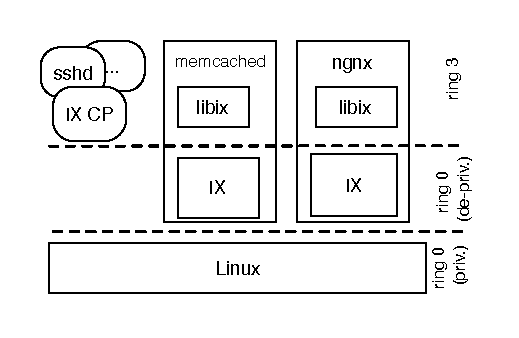
\includegraphics{figs/cp-dp.eps}
\centering\caption{Protection and separation in \ix.}
\label{fig:cp-dp}
\end{centering}
\end{figure}


\begin{figure*}
\subfloat[Protection and separation of control and data plane]{
\label{fig:cp-dp}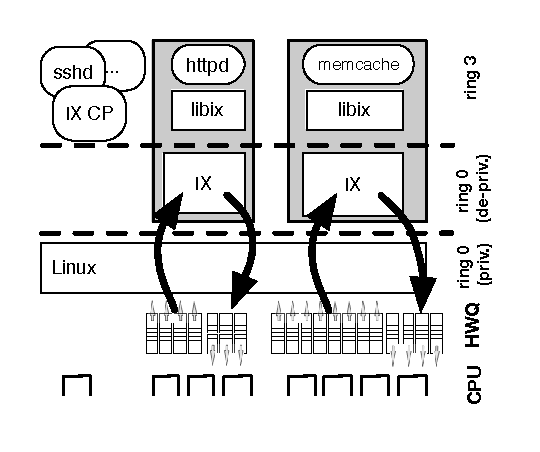
\includegraphics{figs/bigpicture}}
\hspace*{.5em}
\subfloat[Interleaving of protocol processing and application execution]{
\label{fig:dataplane}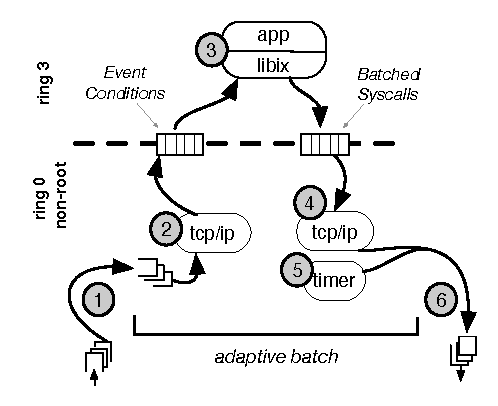
\includegraphics{figs/pipeline-2}}

\caption{The IX dataplane operating system}
\label{fig:ix}
\end{figure*}


\begin{comment}
\dm{Make clear how this corresponds to
    figure 1---i.e., that the dotted line separates ring 3 from VMX
    non-root ring0.  Also, this diagram makes it look like there are
    big queues, contradicting the process to completion idea.  Maybe
    use a different abstraction for queues vs.\ batches (which I
    assume is what is being depicted across the dotted line).  Finally
    the diagram should close the loop in some way.  I.e., do you go
    straight from 5 (really 6 should be depicted0 back to 1, or do you
    invoke a scheduler or check if you need to relinquish the core at
    that point?}}
\end{comment}



\myparagraph{Native, zero-copy API with explicit flow control:} We do
not expose or emulate the POSIX API for networking.  Instead, the
dataplane and the application communicate asynchronously with each
other via messages stored in
memory. % ~\cite{DBLP:conf/osdi/HanMCR12,DBLP:journals/cacm/Rizzo12}
The API meets the commutativity rule and allows for a true zero-copy
operation in both directions, which improves both latency and packet
rate. The dataplane and application cooperatively manage the message
buffer pool. Incoming packets are mapped read-only into the
application, which may hold onto message buffers and return them to
the dataplane at a later point.  The application sends to the
dataplane scatter/gather lists of memory locations for transmission
but, since contents are not copied, the application must keep the
content immutable until the peer acknowledges reception. The
data plane enforces flow control correctness and may trim transmission
requests that exceed the available size of the sliding window, but
the application controls transmit buffering.
%Essentially, the API directly, but safely, exposes flow control to
%applications.

\myparagraph{Flow consistent, synchronization-free processing:} We use
multi-queue NICs with RSS support to provide flow-consistent hashing
of incoming traffic to distinct hardware queues. Each hardware
thread serves a single receive and transmit queue per NIC, eliminating
the need for synchronization and
coherence traffic between cores in the networking stack.  The control
plane establishes the mapping of RSS flow groups to queues to balance
the traffic among the hardware threads.  Similarly, memory management
is organized in distinct pools for each hardware thread. The absence
of a POSIX socket API eliminates the issue of the shared file
descriptor namespace in multithreaded
applications~\cite{DBLP:conf/sosp/ClementsKZMK13}. Overall, the \ix
dataplane design scales well with the increasing number of cores in
modern servers, which improves both packet rate and latency. This
approach does not restrict the memory model for applications, which
can take advantage of coherent, shared memory to exchange information and
synchronize between cores.

